\stopallthesefloats{}

\subsection{Dynamic Verification of Cache Coherence}
\begin{figure}
\begin{center}
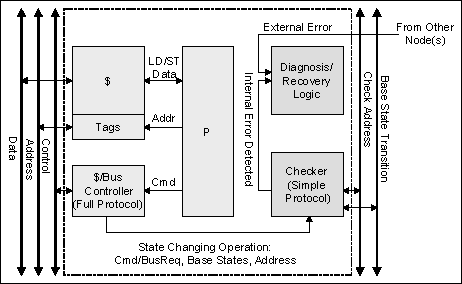
\includegraphics[width=0.7\textwidth]{\chapterdirectory/figure/handling_it/dynamic_verification.pdf}
\end{center}
\caption{Overview of the altered cache, as seen in \cite{Cantin2004DynamicVO}.}%
\label{fig:handling_it:dynamic_verification}
\end{figure}

\cite{Cantin2004DynamicVO} proposes a strategy to implement fault detection in
cache coherence systems, addressing both permanent and temporary issues by
adding hardware (See Figure~\ref{fig:handling_it:dynamic_verification}) that
replicates a simplified version of the cache coherence logic and tests it for
consistency with the real one.

The approach proposed by \cite{Cantin2004DynamicVO} recommends the addition
of a new interconnect dedicated to the validation of the cache coherence
protocol, to avoid disrupting the existing one. This new interconnect is solely
used by caches to broadcast that they entered a stable state for a given memory
element so as to allow the other caches to check that their local state for that
memory element is not in conflict with the broadcasted one. For example, if a
cache broadcasts that it has reached the $M$ state for a memory element, then
all other caches seeing that broadcast would test that they do not have that
memory element in any state other than $I$.

This new verification performed on each cache partaking in the coherence
protocol requires the addition of some hardware to each cache. In addition to
checking for consistency with the other caches through broadcasts, this new
hardware maintains a simplified version of the coherence state of each memory
element. It does not incorporates transient states and, since it only considers
state changes and whether they allow a given instruction to be performed, the
resulting coherence protocol is that of one operating on an atomic interconnect
with atomic operations (such as the one in Section~\ref{sec:intro_to_msi}).
In effect, the simplified protocol only sees events once the transaction they
were part of has been completed. At that point, it receives address, event,
initial and final stable state and compares these with its own record. To detect
timeout issues, a watchdog is also added to the caches.

Thus, while it requires rather complex hardware modifications,
\cite{Cantin2004DynamicVO} does provide a way to detect the occurrence of errors
in the cache coherence protocol's behavior.

\stopallthesefloats{}
